\documentclass[a4paper,parskip]{scrartcl}
\usepackage[usenames,dvipsnames,svgnames,table]{xcolor}
\usepackage[utf8]{inputenc}
\usepackage[ngerman]{babel}
\usepackage{amsmath}
\usepackage{enumerate}
\usepackage{textcomp}
\usepackage{fancyhdr}
\usepackage[a4paper]{geometry}
\usepackage{amsthm}
\usepackage{amsfonts}
\usepackage[version=3]{mhchem}
\usepackage{graphicx}


\author{Sven Jandura} 
\title{Svens Fit Sachen}

\geometry {
  top=0.75in,
  headsep=3ex,
  bottom=0.75in,
}

\fancypagestyle{plain}{
  \fancyhf{}
  \fancyhead[L]{Sven Jandura}
  %\fancyhead[C]{} %Center
  \fancyhead[R]{Seite \thepage}
}

\renewcommand{\headrule}{\color{Black}\hrule height\headrulewidth\hfill}
\pagestyle{plain}

\let\stdsection\section\renewcommand\section{\newpage\stdsection}

\newtheorem{mydef}{Definition}
\newtheorem{mythe}{Satz}


\begin{document}

\maketitle

\tableofcontents

\section{Absorbtionsspektrum}

Es wird werden die Peaks des Referenzresonator gegen die Zeit aufgetragen und mit einem Polynom dritter Ordung gefitted, um die Nichtlinearitär der Verstimmung des Lasers zu korrigieren.

\begin{figure}[h]
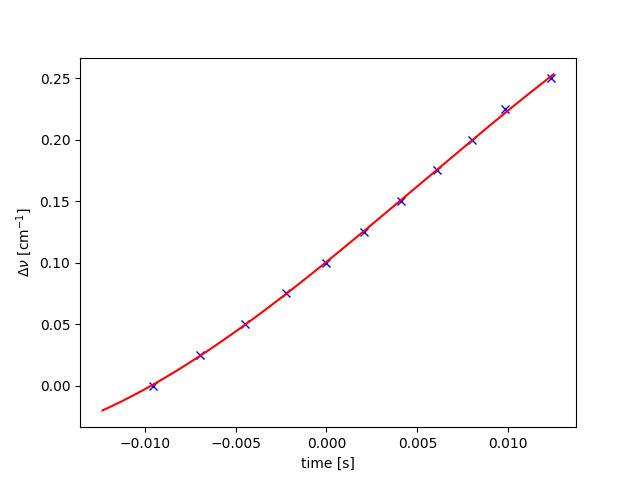
\includegraphics[scale = 0.5]{./absorbtion/frequencyCorrection}
\end{figure}

Das Absorbtionsspektrum wird mit 4 


More to Come

\end{document}

